\icode{E-MCC-SI-L3-261022-002}
如图所示，光滑圆轨道固定在竖直面内，\(BC\)是轨道的水平直径，\(O\)为圆心，一个小球静止在轨道的最低点\(A\)。现给小球水平向左的初速度，小球沿圆轨道向上运动到\(D\)点时刚好离开圆轨道，此后小球恰能通过\(E\)点，\(E\)为\(O\)点上方与\(D\)等高的位置，\(OD\)与水平方向的夹角为\(\theta\)，不计小球的大小，则\paren[]

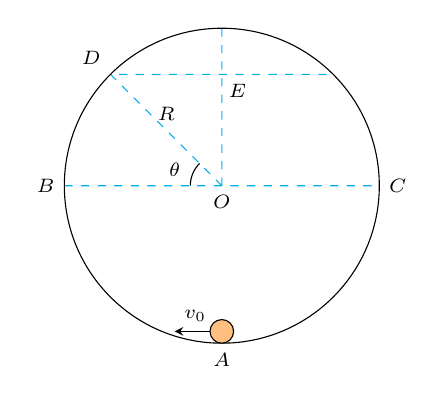
\begin{tikzpicture}[>=stealth,font=\scriptsize]
	\draw[dashed,cyan] (-2,0)node[left,black]{\(B\)}--(2,0)node[right,black]{\(C\)} (0,2)--(0,0)node[below,black]{\(O\)} (0,0)--node[above,black]{\(R\)}({-sqrt(2)},{sqrt(2)})node[above left,black]{\(D\)}--({sqrt(2)},{sqrt(2)});
    \draw (0,0) circle(2);
	\draw (-.4,0) arc(180:135:.4);
	\node at(-.6,.2){\(\theta\)};
	\draw[->] (0,-1.85)--(-.6,-1.85)node[above right]{\(v_0\)};
	\draw[fill=orange!50] (0,-1.85) circle(.15);
	\node at(0,-2)[below]{\(A\)};
	\node at(.2,1.2){\(E\)};
\end{tikzpicture}
\begin{choices}
	\item\(\theta =\)\,\qty{30}{\degree}
	\item\(\theta =\)\,\qty{37}{\degree}
	\item\(\theta =\)\,\qty{45}{\degree}
	\item\(\theta =\)\,\qty{53}{\degree}
\end{choices}
\begin{answer}
    
\end{answer}